%%
%% 2019 07 04 Ph. G. Freimann
%%
\newpage
\section{Binomische Formeln}\index{Formeln!binomische}\index{Binomische Formeln}

\sectuntertitel{2: Zwei, bi-, di-, zwie-, doppel, binär, duo, dual,
Boole'sch, paar, stereo, sekund-, ...\footnote{Zürich unterscheidet die Zahl
2 je nach Geschlecht: «zwoo Fraue», «zwéé Mane» und «zwäi Chinde»}}

\theorieTALS{16}{1.3.1}
\theorieGESO{29}{2.2.1}

Einführendes Youtube-Video:\texttt{youtu.be/nSmlfe-ftTo} und \texttt{youtu.be/zYVY0nmGnbE} und eine Anwendung
\texttt{youtu.be/k-dGzlWNblo}

%%%%%%%%%%%%%%%%%%%%%%%%%%%%%%%%%%%%%%%%%%%%%%%%%%%%%%%%%%%%%%%%%%%%%%%%%%%%%%%%%
\subsection*{Lernziele}

\begin{itemize}
\item Erste:  $(a+b)^2$ 
\item Zweite: $(a-b)^2$
\item Dritte: $(a+b)(a-b)$
\item $(a+b)^3$, $(a+b)^4$

%%  \item Polynomdivision

\end{itemize}
\newpage


\subsection{Binomische Formeln}\index{Formeln!binomische}
Es gilt:

\TNT{4}{
  $(a+b)\cdot(c+d) = \overbrace{(a+b)}^{X} \cdot (c+d)
  =X(c+d)
  =Xc + Xd
  =(a+b)c + (a+b)d
  =ac + ad + bc + bd$
}%% END TNT

Daraus folgen die drei binomischen Formeln
\begin{gesetz}{Binomische Formeln}{}
$$(a+b)^2 = a^2 + 2ab +b^2$$
$$(a-b)^2 = a^2 - 2ab +b^2$$
$$(a+b)(a-b) = a^2 - b^2$$
\end{gesetz}

Graphischer Beweis der 1. binomischen Formel:

%% Für Millimeterpapier siehe auch hier:
%%     http://www.texample.net/tikz/examples/graph-paper/


\TNT{5.2}{%
\raisebox{-1cm}{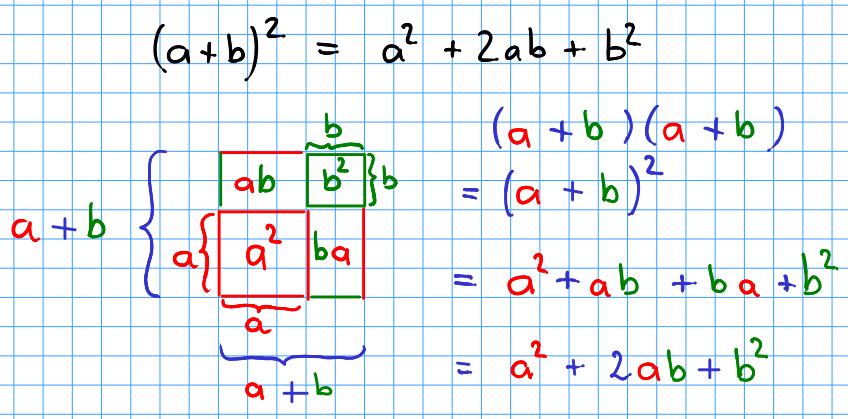
\includegraphics[width=12cm]{allg/alg/img/a_plus_b_zum_quadrat.png}}%
}%% END TNT


%Mit diesem Wissen lassen sich einige Summen einfacher ausklammern:
%\vspace{4cm}
%\TRAINER{
%  $$49 - x^2 = (7-x)\cdot(7+x)$$
%  $$a^2 -16a + 64 = (a-8)^2$$
%}

\TALS{
\subsection{Pascalsches Dreieck}\index{Pascalsches
  Dreieck}\index{Dreieck!Pascalsches}

Berechnen Sie $(a+b)^4$:

\noTRAINER{\noteLines{8}}
\TRAINER{$a^4 + 4a^3b + 6a^2b^2 + 4ab^3 + b^4$}

Zeichen Sie das Pascalsche Dreieck:
\begin{center}
\begin{tabular}{cccccccccccc}\\
  &   &     &     &     & 1   &     &     &     &     &    & \\
  &   &     &     & 1   &     & 1   &     &     &     &    & \\  
  &   &     & 1   &     & 2   &     & 1   &     &     &    & \\
  &   &  1  &     & 3   &     & 3   &     & 1   &     &    & \\
  & 1 &     & ... &     & ... &     & ... &     & ... &    & \\ 
1 &   & ... &     & ... &     & ... &     & ... &     & ...&  
\end{tabular}
%\noTRAINER{\vspace{3cm}}
\end{center}
}


\TALS{\newpage}
\subsection*{Aufgaben}
\TALSAadB{16}{21a) d), 22a) b) e)}

\TALSAadB{17}{23a) 24a)}

\GESOAadB{36ff}{ 19. b) d) h) 20. a) b) c) d) 21. a) 23. a) 24. a)
25. b) e) Optional: 27. c)}

